\subsection{The TorPath Protocol}

\subsubsection{Overview}

We introduce the TorPath protocol for assigning Tor circuits to clients. It
overrides Tor directory servers with \textit{assignment servers}, which form
decentralized \textit{consensus groups}. The protocol guarantees that no
participant on a circuit can identify all other participants, and that each
circuit includes a publicly verifiable signature. We use TorPath to ``sign''
each TorCoin, so that anyone can verify its authenticity.

\subsubsection{Requirements}

The TorPath protocol adheres to the following constraints:

\begin{itemize}   
\item No client can generate its own circuit.   
\item Every circuit has a unique, publicly-verifiable signature.   
\item No client can know the circuit of another client. 
\end{itemize}

\subsubsection{Protocol Description}

\paragraph{Group Formation}

A consensus group is formed when a majority of the Assignment Servers come
together to assign circuits to clients. Thus, if there are 10 Assignment Servers
in the network, atleast 6 of them must collectively form a group.  The size of
each anonymity group can be modulated to be a number n, i.e., the group waits
until there are n clients to proceed to the next stage. Different groups can
have different values of n to provide different levels of anonymity to different
clients. Groups with larger values of n would provide a larger anonymity set, at
the expense of higher connection times.

The steps in group formation are: 
\begin{enumerate} 
\item Some Assignment Servers come together to form a group. Each server shares 
its own public key with all the others. 
\item Clients connect to an assignment server that is accepting clients and 
download the public keys of all the assignment servers in the group.
\item Relays connect to an assignment server and download the public
keys of all assignment servers in the group. 
\item Clients generate a temporary public and private key-pair. The public key 
is then onion-encrypted with all the servers' public keys and sent to the server.
\end{enumerate}

\begin{figure}[htbp]
  \centering
  \subfloat[]{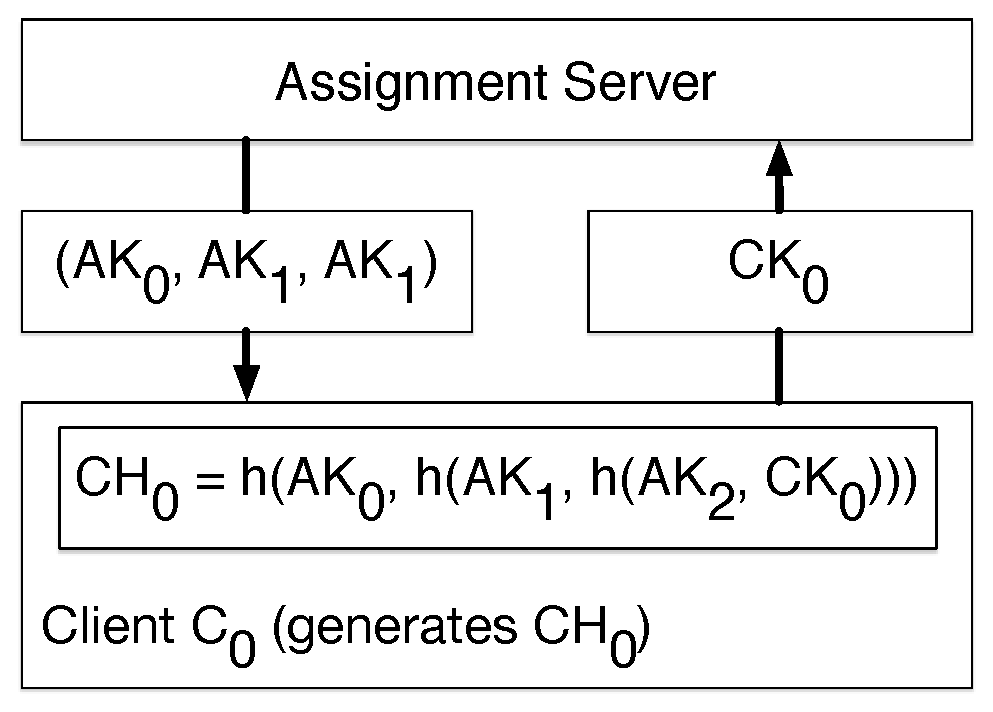
\includegraphics[width=.49\textwidth]{group_formation_2.pdf}}
  \subfloat[]{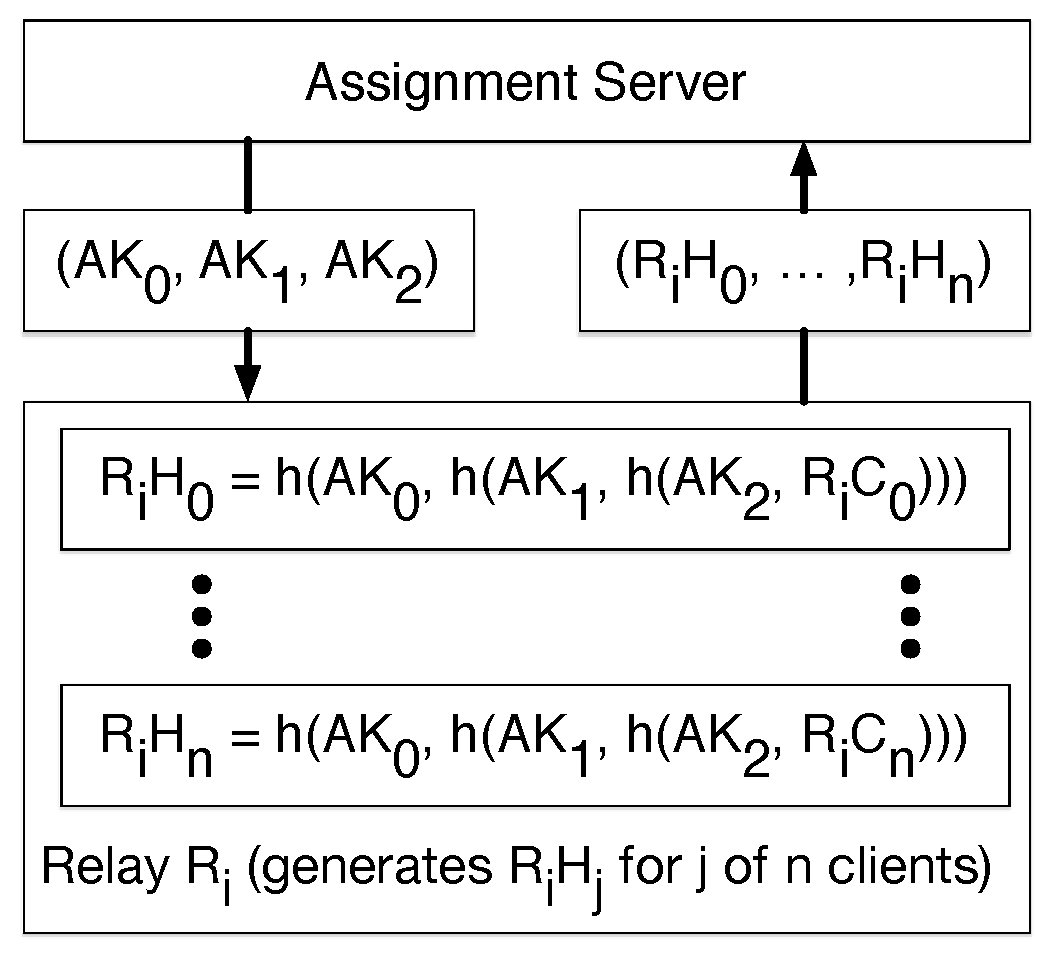
\includegraphics[width=.49\textwidth]{group_formation_3.pdf}}
  \caption{Group Formation (a) Servers form a consensus group. 
    (b) Clients onion-encrypt their public keys. 
    (c) Relays onion-encrypt multiple public keys.}
  \label{rfidtag_testing}
\end{figure}

\paragraph{Verifiable Shuffle}

In most cases, the number of available relays will be less than that of clients 
in a group. 
\begin{enumerate} 
\item Each relay chooses which position(s) it wants to be in.
\item For each position, the server asks each participating relay to generate a 
number of keypairs
such that the total number of keypairs is equal to the number of clients. Thus,
the cumulative number of generated keypairs over all the positions is $3n$.
\item Each of the public keys is onion-encrypted with all the public keys of all the 
servers and sent to them. The servers, thus, have separate lists of entry, middle
and exit relay keys, each of size $n$.
\end{enumerate}

The servers then perform a separate verifiable shuffle (eg. using the Neff
Shuffle\cite{neff2001verifiable}) on each kind of key: client keys, entry relay
keys, exit relay keys and middle relay keys. The output of each shuffle is a
verifiable, shuffled list of $n$ keys, as described in FIGURE. 

\begin{figure}[htb]
\centering
\hspace{\fill}%
\subfloat[htb][left]{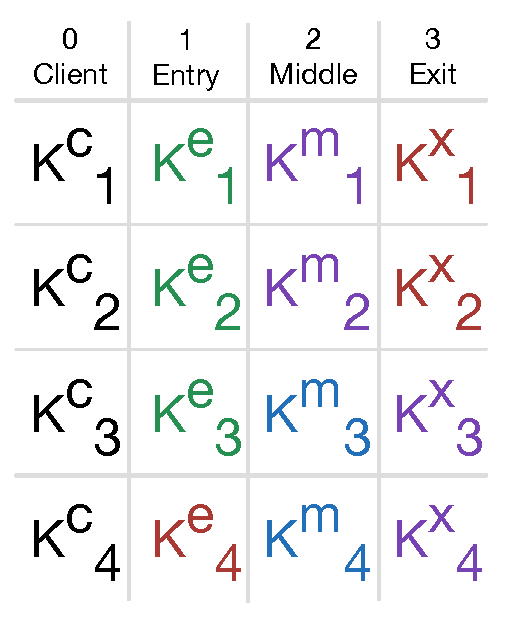
\includegraphics[scale=0.4]{shuffle_1.pdf}}
\hspace{\fill}%
\subfloat[htb][right]{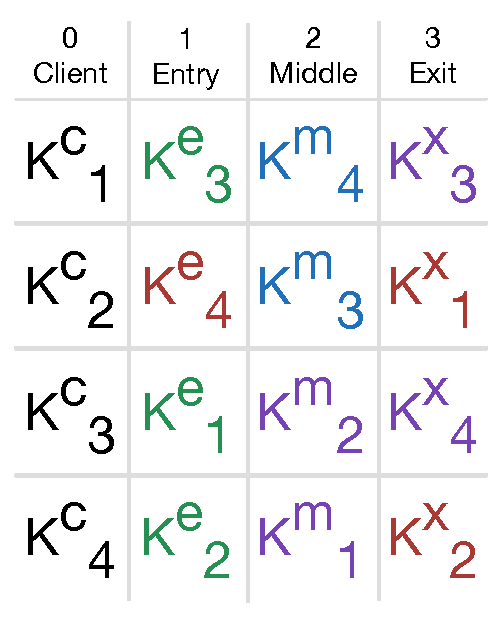
\includegraphics[scale=0.4]{shuffle_2.pdf}}
\hspace*{\fill}%
\caption[bla]{foobar}
\end{figure}

We may represent the results of the shuffle as a $n \times 4$ matrix $M$, with
each row representing a client and its three relays in the order: entry, middle
and exit. This output matrix is also published in a publicly acessible log and
signed by all the servers participating in the group.usu

\paragraph{Path Lookup}
Once the shuffle is completed and published, all clients and relays can look up
their own keys in their respective columns. They can also find the public keys 
of all the other participants in their path. Using this information, they send 
their IP Address information onion-encrypted in the message format outlined in
table \ref{table:message_format}.

\begin{table}
  \begin{tabular}{ c || p{9cm} }
  \hline
  Sender & Message Tuple \\ \hline
  Client & ($K_{i}^{C}$, {$IP_{i}^{C}$ encrypted with the public key of its 
  entry relay}) \\ \hline
  Entry relay & ($K_{i}^{E}$, {$IP_{i}^{E}$ encrypted with the public key of 
  its corresponding client}, {$IP_{i}^{E}$ encrypted with the public key of 
  its corresponding middle relay}) \\ \hline
  Middle relay & ($K_{i}^{M}$, {$IP_{i}^{M}$ encrypted with the public key of 
  corresponding entry relay}, {$IP_{i}^{M}$ encrypted with the public key of 
  corresponding exit relay}) \\ \hline
  Exit relay & ($K_{i}^{X}$, {$IP_{i}^{X}$ encrypted with the public key of 
  corresponding middle relay}) \\ \hline
  \end{tabular}
  \caption{Each participant in a circuit sends its message 
  tuple onion-encrypted to the server. The superscripts refer to the position 
  of the relay in the circuit and the subscript is the $i^{th}$ row of $M$.}
  \label{table:message_format}
\end{table}

\begin{figure}
\centering
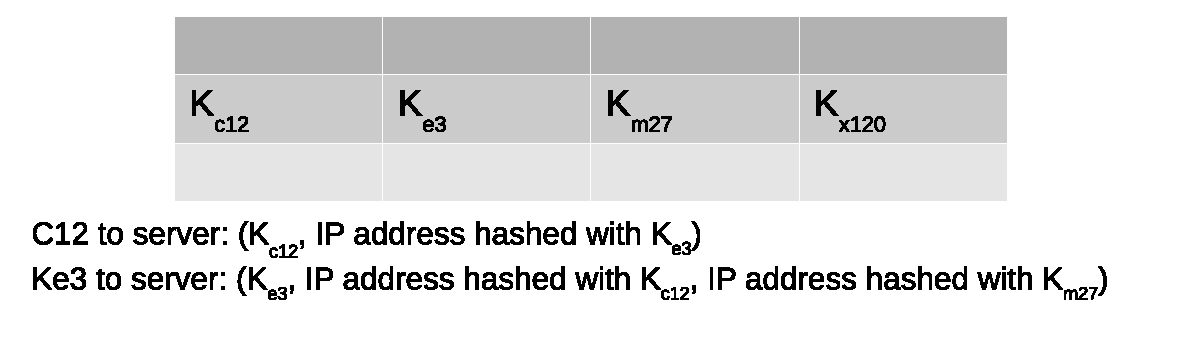
\includegraphics[scale=0.5]{address_lookup.eps}
\caption{An Example Path Lookup}
\end{figure}

These tuples are shuffled by the servers again. Each client and relay can then 
decrypt the IP address of their neighbours using their own public key.

The clients then have a circuit which they can use to communicate using the Tor 
protocol.

\paragraph{Circuit Signature}
The Circuit Signature of the ith circuit in a shuffle is the product of the keys
in row i of the matrix:
$RS_i = M_{i0} \times M_{i1} \times M_{i2} \times M_{i3}$
This key, using El Gamal encryption, can be used to verify the proof-of-work.

\subsubsection{Circuit Anonymity} 
The TorPath protocol guarantees that no single server can be aware of the entire
circuit of any client. 


% % Next we will descibe the consensus groups and Neff shuffle in more detail.

% % \begin{figure}[H] %   \centering %
% 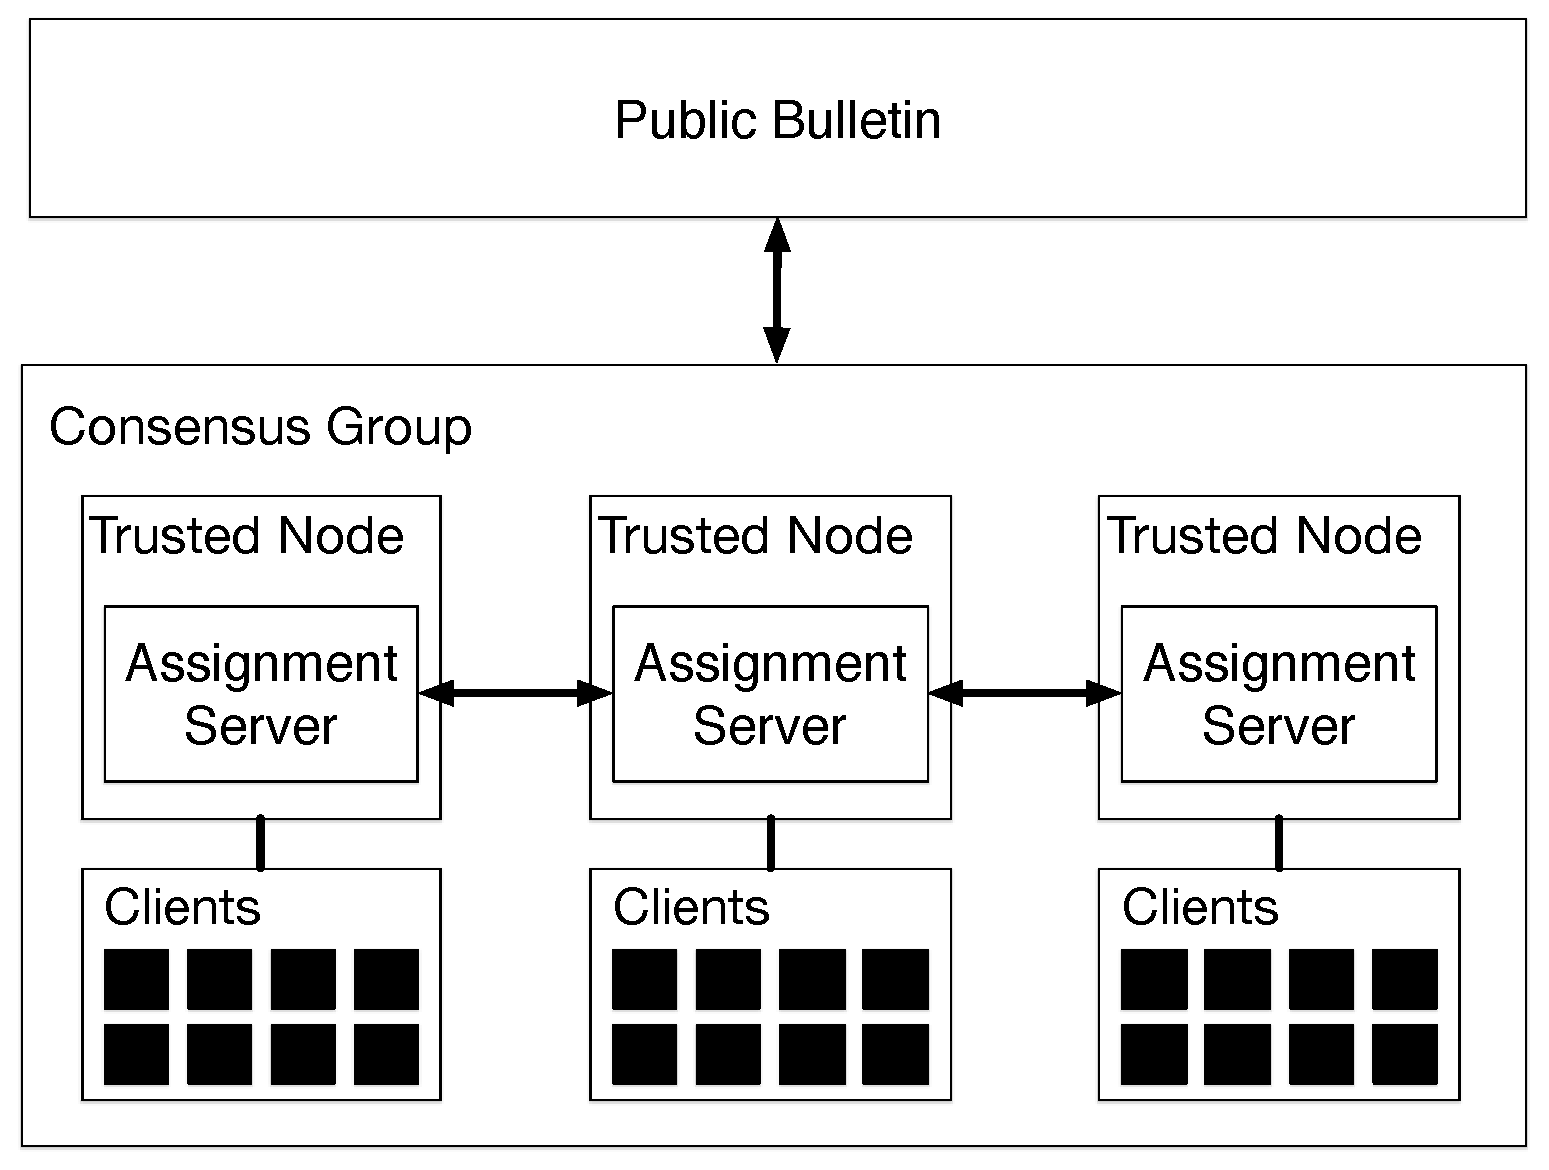
\includegraphics[scale=0.3]{torpath_grouping.pdf} %   \caption{TorPath Consensus
% Group Formation.} % \end{figure}

% % \subsubsection{Group Formation} % An assignment server joins a group when it
% reaches a sufficient number of clients. In practice, we expect the number to be
% modulated so that groups are being created every 10 seconds or so. To ensure
% diversity, groups must include a majority of the assignment servers on the
% network. For example, if there are ten of assignment servers on the entire
% network, a consensus group requires at least six.

% % Once a consensus group exists, it splits into three decentralized shuffle
% % sets, each responsible for assigning a different relay to clients. An
% % $n$-client shuffle set has $n$ rows, each pointing to a possible relay. For
% % example, shuffle sets $s_0$, $s_1$, and $s_2$ could be responsible for
% % assigning entry, middle, and exit relays to clients.

% % \subsubsection{Neff Shuffles for Circuit Assignment} % Each shuffle set runs a
% Neff shuffle ~\cite{neff2001verifiable} to shuffle its list of $n$ relays, so
% that it can assign each relay $i$ to client $i$. Each client receives a tuple
% $(r_0, r_1, r_2, s)$ specifying the address of entry, middle, and exit relays,
% along with a circuit signature.

% % \begin{figure} %   \centering %
% 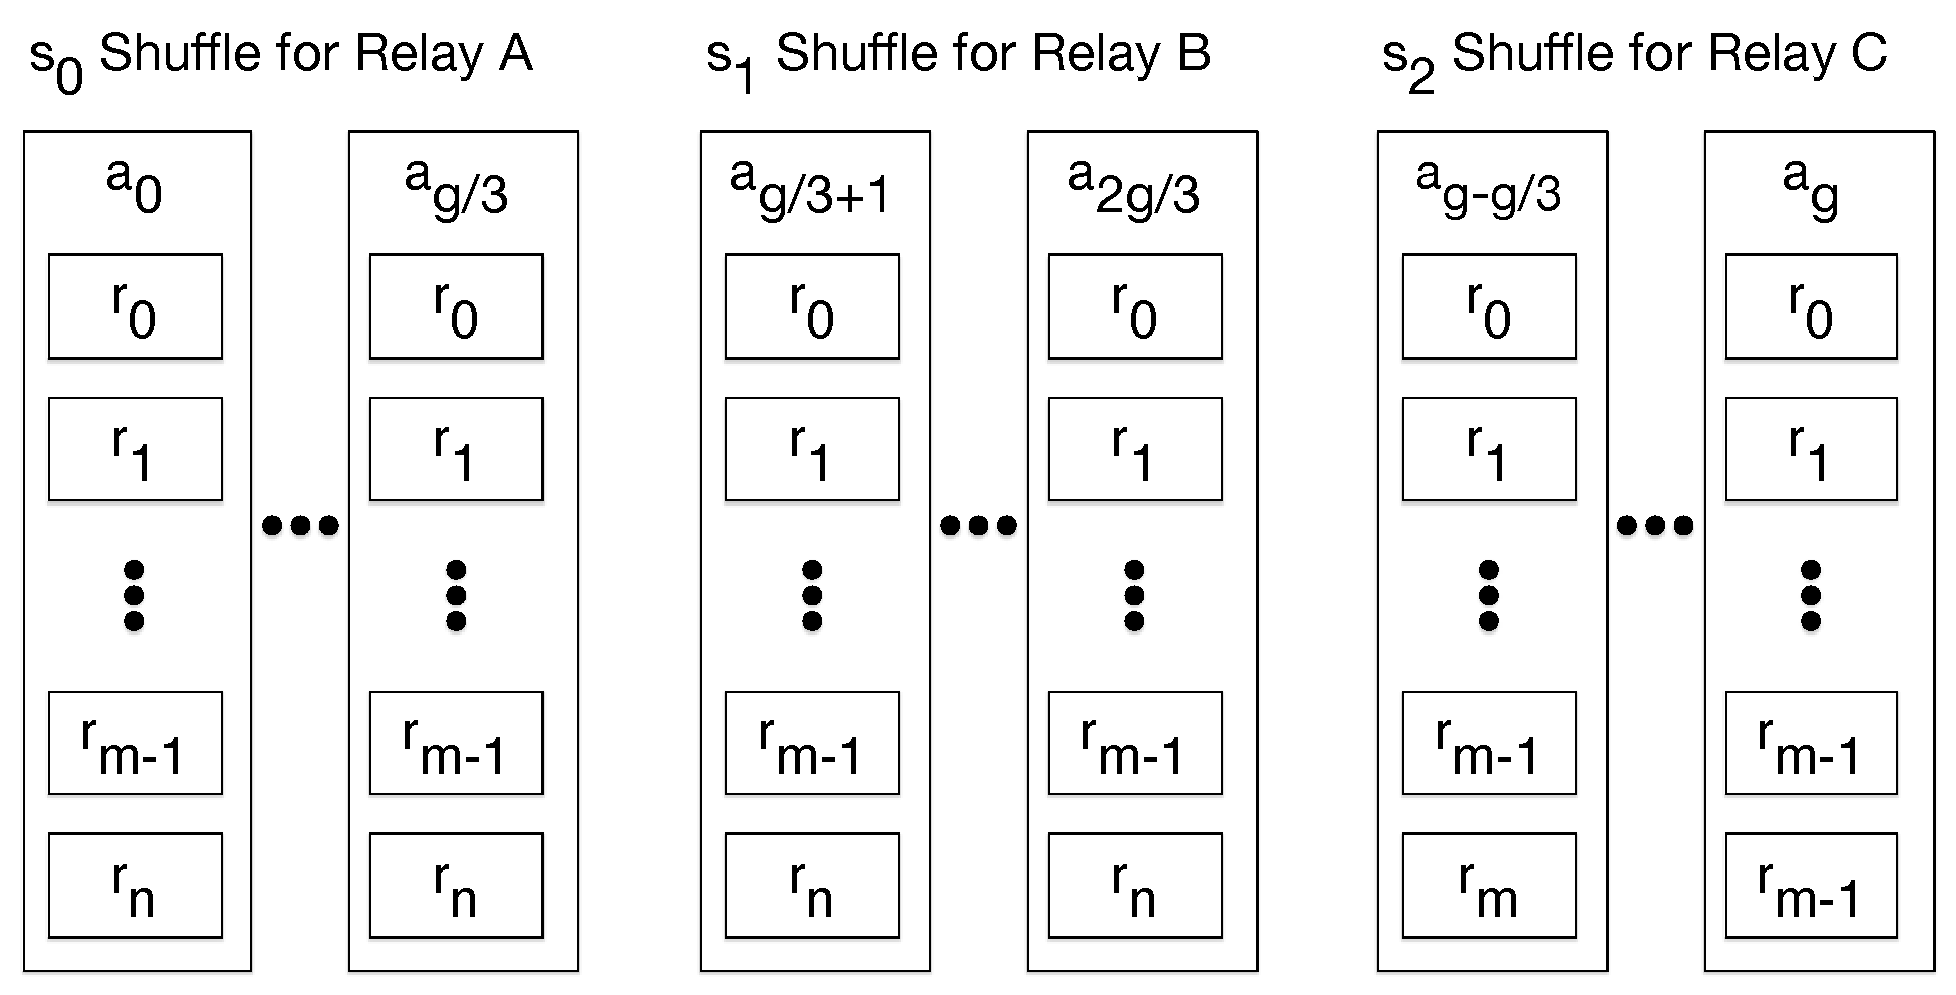
\includegraphics[scale=0.3]{torpath_shufflesets.pdf} %   \caption{Each Shuffle
% Set carries out its own Neff shuffle to determine one part of the path.} %
% \end{figure}

% % \subsubsection{TorCoin Verification} % Assignment servers input circuit
% signatures into a cryptographic accumulator, and publish that list of
% accumulators. Anyone can verify that a circuit existed at least once, simply by
% searching for a signature.

% % \subsubsection{Decoupled Protocol} % The TorPath protocol only replaces
% directory servers. Therefore, implementing it does not require modifying any Tor
% code. So clients can use the TorPath protocol for circuit assignment then
% communicate using the existing Tor protocol.
